\documentclass[12pt, aspectratio=169]{beamer}
\usetheme{Madrid}
\usefonttheme{professionalfonts}
\usepackage{fontspec}

\setsansfont{InterDisplay}[
  UprightFont=*-Regular,
  ItalicFont=*-Italic,
  BoldFont=*-Bold,
  BoldItalicFont=*-BoldItalic,
  RawFeature={+cv05}
]
\setmonofont{Adwaita Mono}
\renewcommand{\small}{\fontsize{11}{13}\selectfont}
\renewcommand{\normalsize}{\fontsize{12}{14}\selectfont}
\renewcommand{\large}{\fontsize{14}{17}\selectfont}
\newcommand{\rcode}[1]{{\small\texttt{#1}}}
\newcommand{\bcode}[1]{{\small\texttt{\textbf#1}}}

\title{\addfontfeatures{RawFeature={+cv08}}Astroinformatics I\\\vspace{2.5mm}
Project Presentation}

\subject{Astroinformatics I}
\author{Jos\'e Batista-Mendoza}
\institute{CITEVA, Universidad de Antofagasta}
\date{\today}

\setbeamertemplate{navigation symbols}{}
\setbeamertemplate{footline}{}

\begin{document}

  \begin{frame}[t]
    \titlepage
  \end{frame}

  \begin{frame}[t]{Table of Contents}
    \large\textbf\tableofcontents
  \end{frame}
  
  \section{Introduction}
  \begin{frame}[t]{Introduction}
    \textbf{Motivation:} \vspace{2.5mm}
    \begin{itemize} \large
      \item In modern astronomy, theoretical knowledge must be coupled with strong computational skills. \vspace{1mm}
      \item Astroinformatics is precisely this intersection: applying informatics tools to astronomical data. \vspace{1mm}
      \item Bridge the gap between classroom concepts and their tangible application in real-world data handling and analysis. \vspace{1mm}
      \item Show how the fundamental computational principles provided in the course become powerful instruments for astronomical discovery.
    \end{itemize}
  \end{frame}

  \begin{frame}[t]{Introduction (Cont.)}
    \textbf{Course Overview:} \vspace{2.5mm}
    \begin{itemize}
      \item Astroinformatics I covered a comprehensive range of essential computational topics. \vspace{1mm}
      \item From foundational Linux command-line operations and shellfor data management, \vspace{1mm}
      \item Through core Python programming for data manipulation and analysis, \vspace{1mm}
      \item To specialized astronomical libraries (\rcode{astropy}, \rcode{pandas}, \rcode{numpy}, \rcode{matplotlib}) for specific data challenges. \vspace{1mm}
      \item Finally, integrating crucial software engineering principles for robust and reproducible work. \vspace{1mm}
      \item The course emphasized hands-on learning through lectures, tutorials, and graded practices.
    \end{itemize}
  \end{frame}

  \begin{frame}[t]{Introduction (Cont.)}
    \textbf{Presentation Goal:} \vspace{2.5mm}
    \begin{itemize} \large
      \item The primary goal is to illustrate how the theoretical and practical concepts from Lectures and Tutorials were directly applied. \vspace{1mm}
      \item This presentation will walk through key examples from the \textbf{graded practices (Practices 1\textendash4)}. \vspace{1mm}
      \item This will highlight the practical implementation of tasks like data cleaning, transformation, analysis, visualization, and project organization. \vspace{1mm}
      \item Ultimately, showcasing a complete workflow for astronomical data processing.
    \end{itemize}
  \end{frame}

  \section{Practices 1 \& 2: Shell, Linux \& Python Fundamentals}
  \begin{frame}[t]{Shell, Linux \& Python Fundamentals}
    \textbf{Foundation:} Based on Lectures and Tutorials 2\textendash5
    \\\vspace{2.5mm}
    \textbf{Key Concepts Applied:} \\\vspace{2.5mm}
    \begin{itemize}
      \item \textbf{File System Navigation \& Manipulation} \vspace{1mm}
      \begin{itemize}
        \item Identifying files (\rcode{ls}, wildcards like \rcode{*.csv}).
        \item Directory management (\rcode{dirname}, variable expansion).
        \item File creation (\rcode{touch}).
      \end{itemize} \vspace{1mm}
      \item \textbf{Text Processing \& Data Transformation} \vspace{1mm}
      \begin{itemize}
        \item Changing delimiters (\rcode{sed s/,/\ /g}).
        \item Removing columns (\rcode{awk '\{print \$1, \$2, \$3\}'}).
        \item File renaming (\rcode{mv}).
      \end{itemize}
    \end{itemize}
  \end{frame}

  \begin{frame}[t]{Shell, Linux \& Python Fundamentals (Cont.)}
    \textbf{Foundation:} Based on Lectures and Tutorials 2\textendash5
    \\\vspace{2.5mm}
    \textbf{Key Concepts Applied:} \\\vspace{2.5mm}
    \begin{itemize}
      \item \textbf{Shell Scripting Constructs} \vspace{1mm}
      \begin{itemize}
        \item \rcode{for} loops for batch processing.
        \item Conditional statements (\rcode{[ -e "\$csv\_file" ]}, \rcode{if}).
        \item Output Redirection (\rcode{>>}).
      \end{itemize} \vspace{1mm}
      \item \textbf{Python Fundamentals} \vspace{1mm}
      \begin{itemize}
        \item Defining and calling functions.
        \item Performing basic operations, comparisons, data type conversion and string manipulation.
        \item Applying conditional logic (\rcode{if-elif-else}).
        \item Handling command-line arguments (\rcode{sys.argv}).
        \item Incorporating user interaction (\rcode{input()}).
        \item Implementing error handling (\rcode{try-except} blocks).
      \end{itemize}
    \end{itemize}
  \end{frame}

  \begin{frame}[t]{Practice Showcase}
    \begin{itemize}
      \item \textbf{Practice 1:} Listing CSV filenames \vspace{2.5mm}
    \end{itemize}
    \begin{columns}
      \begin{column}{0.5\textwidth}
        \centering
        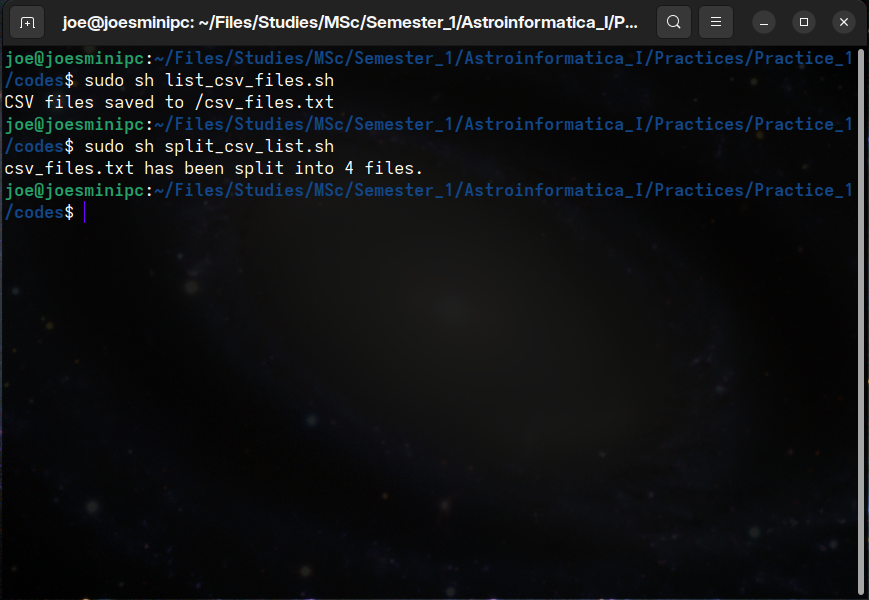
\includegraphics[width=\linewidth]{figures/1-1.png}
      \end{column}
      \begin{column}{0.5\textwidth}
        \centering
        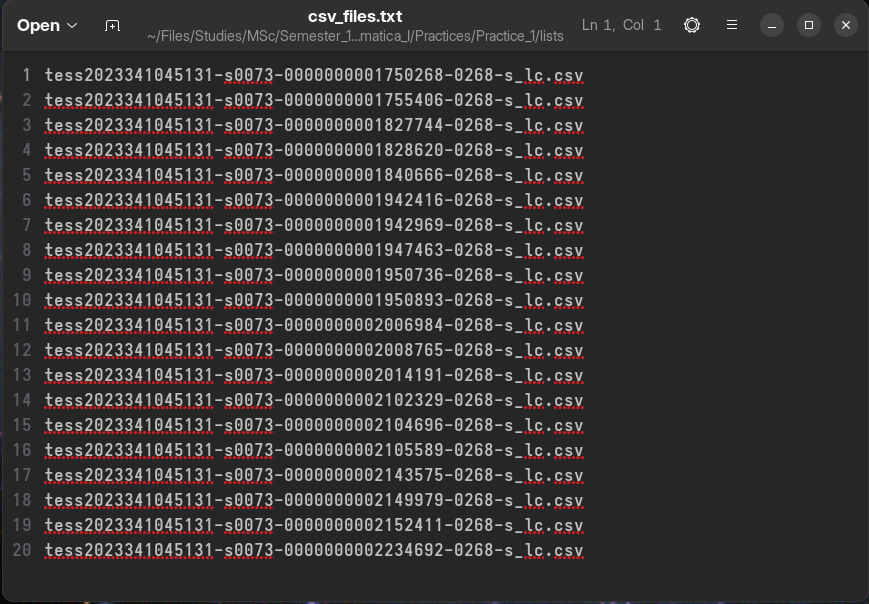
\includegraphics[width=\linewidth]{figures/1-2.png}
      \end{column}
    \end{columns}
  \end{frame}

    \begin{frame}[t]{Practice Showcase (Cont.)}
    \begin{itemize}
      \item \textbf{Practice 1:} Splitting text files \vspace{2.5mm}
    \end{itemize}
    \begin{columns}
      \begin{column}{0.5\textwidth}
        \centering
        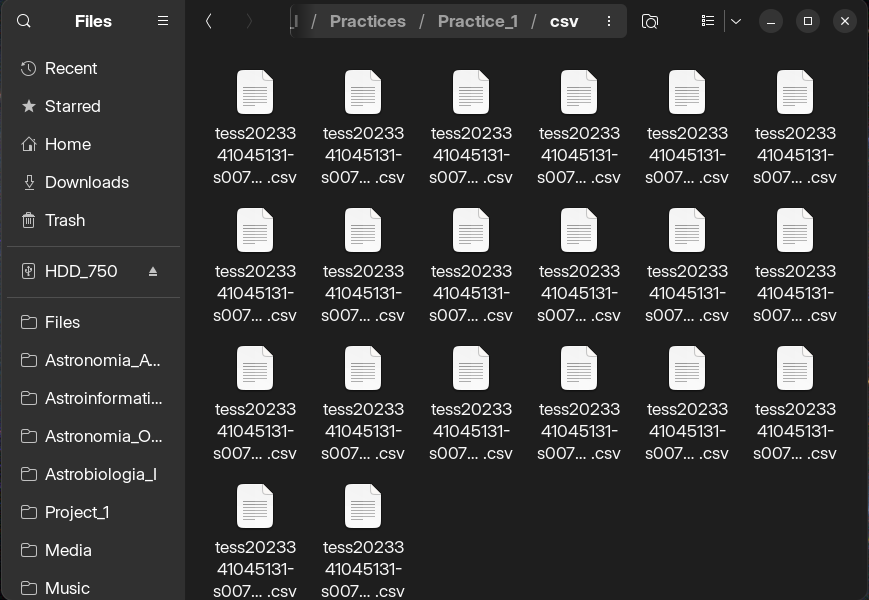
\includegraphics[width=\linewidth]{figures/1-3.png}
      \end{column}
      \begin{column}{0.5\textwidth}
        \centering
        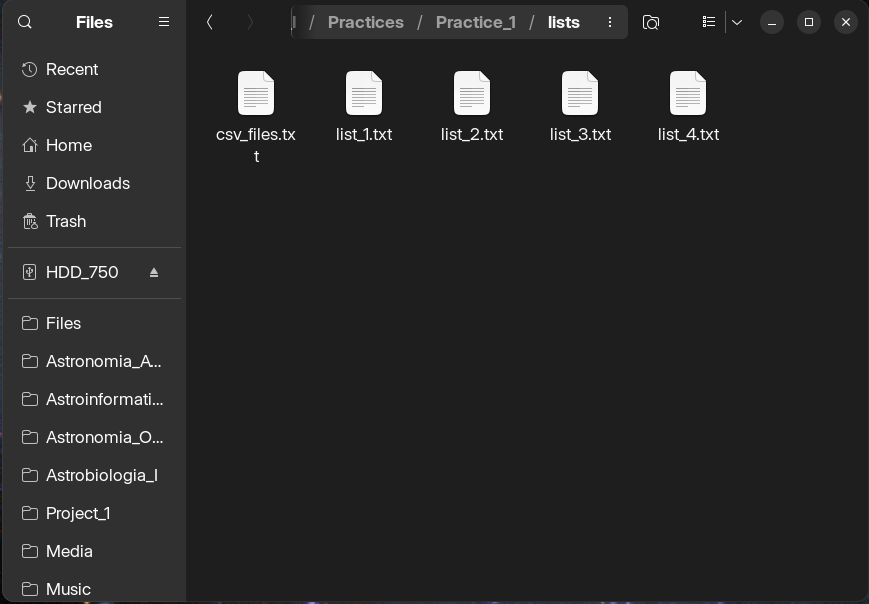
\includegraphics[width=\linewidth]{figures/1-4.png}
      \end{column}
    \end{columns}
  \end{frame}

  \begin{frame}[t]{Practice Showcase (Cont.)}
    \begin{itemize}
      \item \textbf{Practice 2:} Modifying CSV files (delimiter change,
      column removal, and extension change) \vspace{2.5mm}
    \end{itemize}
    \begin{columns}
      \begin{column}{0.5\textwidth}
        \centering
        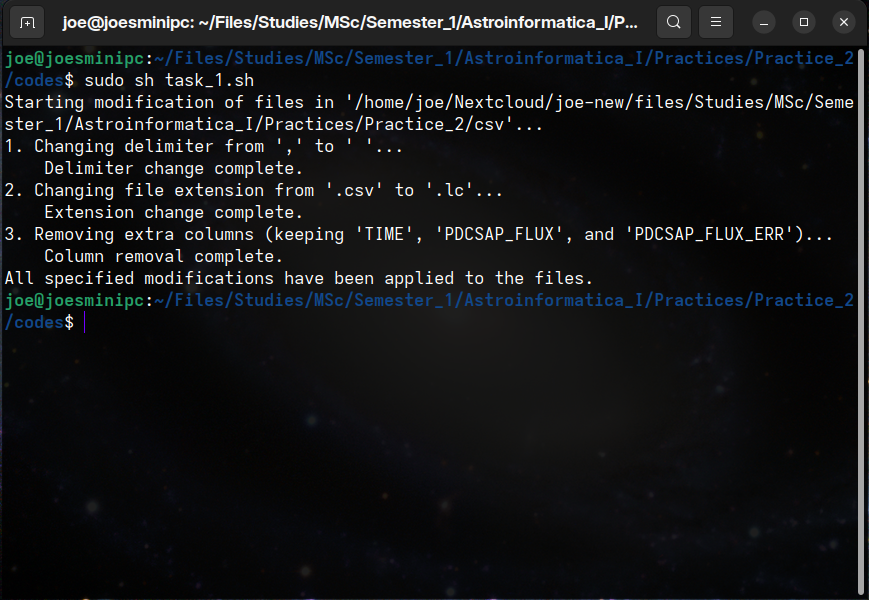
\includegraphics[width=\linewidth]{figures/2-1.png}
      \end{column}
      \begin{column}{0.5\textwidth}
        \centering
        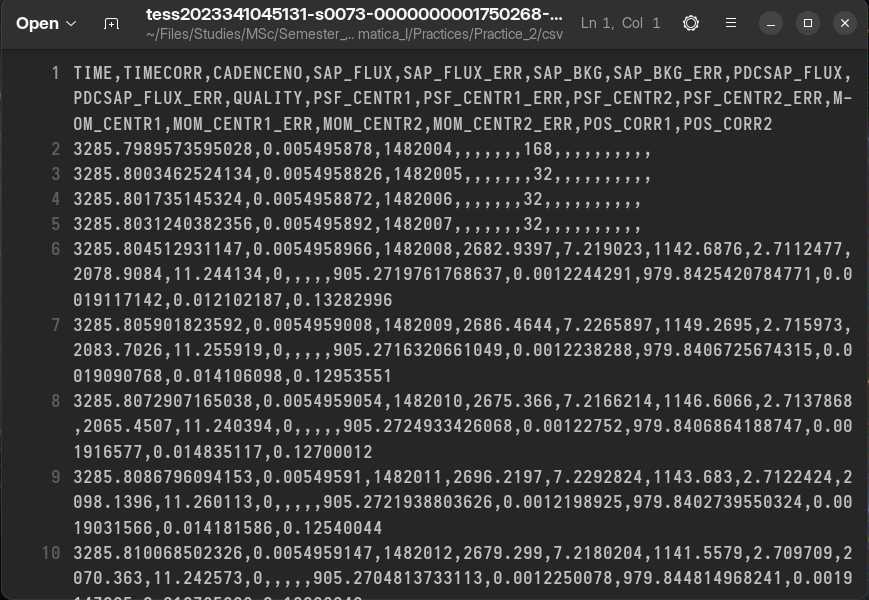
\includegraphics[width=\linewidth]{figures/2-2.png}
      \end{column}
    \end{columns}
  \end{frame}

  \begin{frame}[t]{Practice Showcase (Cont.)}
    \begin{itemize}
      \item \textbf{Practice 2:} Modifying CSV files (Cont.) and basic Python
      scripting \vspace{2.5mm}
    \end{itemize}
    \begin{columns}
      \begin{column}{0.5\textwidth}
        \centering
        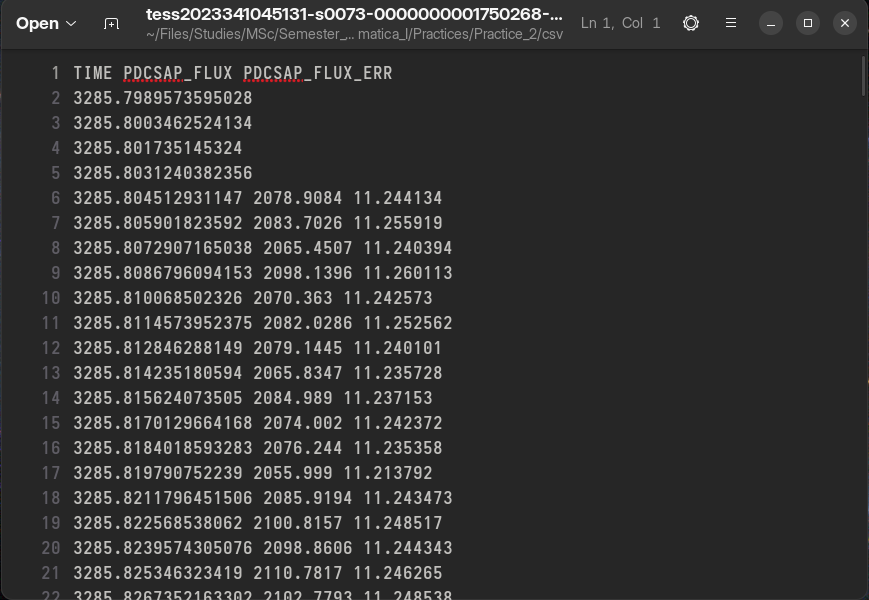
\includegraphics[width=\linewidth]{figures/2-3.png}
      \end{column}
      \begin{column}{0.5\textwidth}
        \centering
        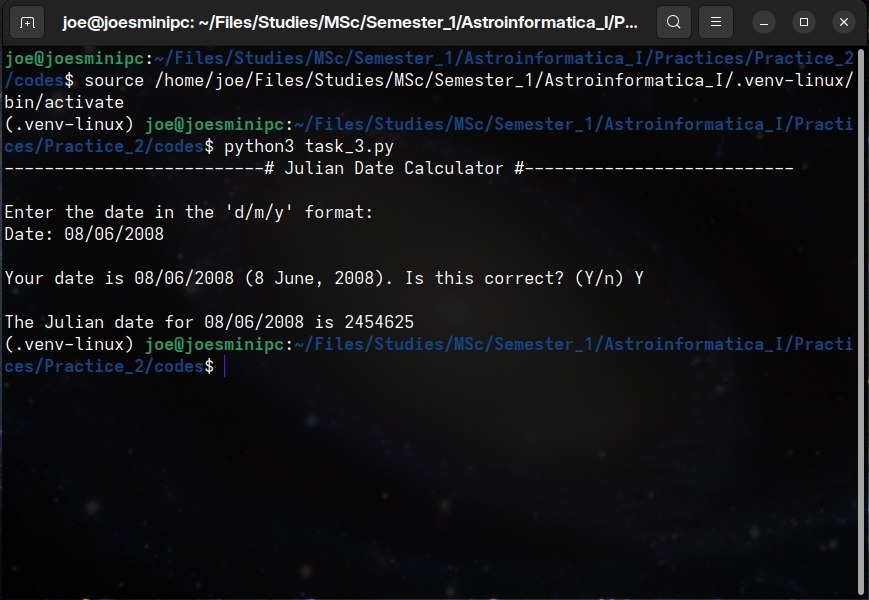
\includegraphics[width=\linewidth]{figures/2-4.png}
      \end{column}
    \end{columns}
  \end{frame}

  \section{Practice 3: Python Programming for Astronomical Data Analysis}
  \begin{frame}[t]{Python for Astronomical Data Analysis}
    \textbf{Foundation:} Based on Lectures and Tutorials 6\textendash7
    \\\vspace{2.5mm}
    \textbf{Key Concepts Applied:} \\\vspace{2.5mm}
    \begin{itemize}
      \item \textbf{Data Manipulation (\rcode{pandas}, \rcode{numpy})} \vspace{1mm}
      \begin{itemize}
        \item Loading and structuring data with \rcode{pandas.DataFrame}.
        \item Numerical operations and statistical analysis (\rcode{numpy}
        for mean, std, median, etc.).
      \end{itemize} \vspace{1mm}
      \item \textbf{Astronomical Data Handling (\rcode{astropy})} \vspace{1mm}
      \begin{itemize}
        \item \rcode{astropy.timeseries.TimeSeries} for light curves.
        \item Time conversion (\rcode{astropy.time.Time}, BTJD to JD TDB, BJD
        to UTC).
        \item Lomb-Scargle periodograms (\rcode{astropy.timeseries.LombScargle}).
      \end{itemize}
    \end{itemize}
  \end{frame}

  \begin{frame}[t]{Python for Astronomical Data Analysis (Cont.)}
    \textbf{Foundation:} Based on Lectures and Tutorials 6\textendash7
    \\\vspace{2.5mm}
    \textbf{Key Concepts Applied:} \\\vspace{2.5mm}
    \begin{itemize}
      \item \textbf{Data Visualization (\rcode{matplotlib})} \vspace{1mm}
      \begin{itemize}
        \item Generating scatter plots with error bars.
        \item Plot customization (titles, labels, legends, colorblind-friendly
        palettes, markers).
        \item Subplots for combined visualizations (light curve + periodogram).
        \item Annotations on plots.
      \end{itemize} \vspace{1mm}
      \item \textbf{Astronomical Concepts:} \vspace{1mm}
      \begin{itemize}
        \item Outlier detection, phase-folding and period finding for TESS light
        curves.
      \end{itemize}
    \end{itemize}
  \end{frame}

  \begin{frame}[t]{Practice Showcase}
    \begin{itemize}
      \item \textbf{Practice 3:} Processing TESS light curves (raw plotting and
      outlier detection)
    \end{itemize}
    \centering
    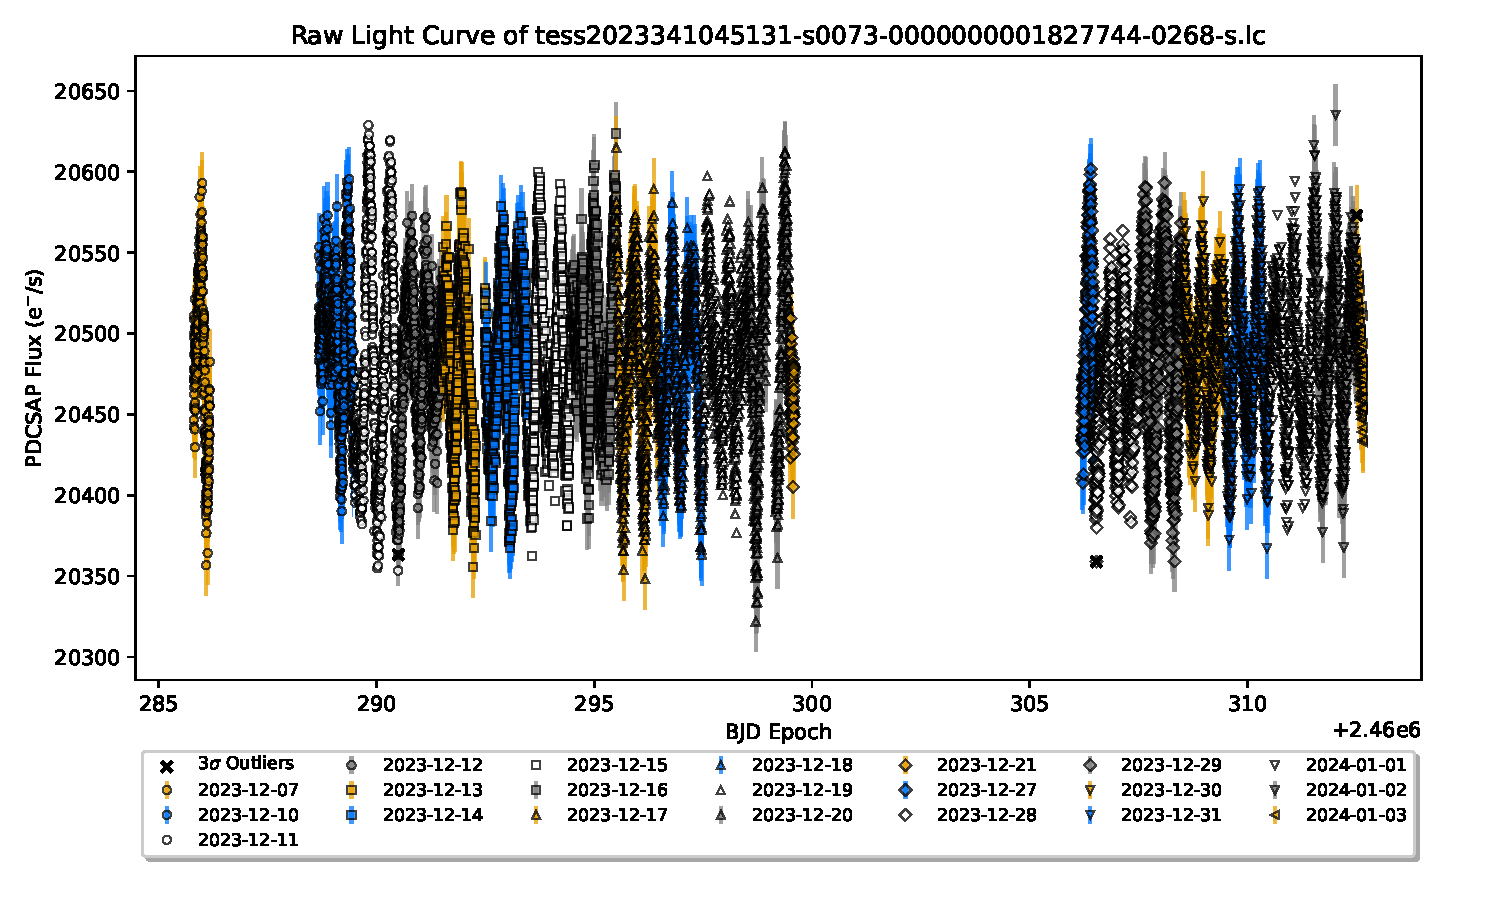
\includegraphics[width=1.35\textheight]{figures/3-1.pdf}
  \end{frame}

  \begin{frame}[t]{Practice Showcase (Cont.)}
    \begin{itemize}
      \item \textbf{Practice 3:} Processing TESS light curves (phase-folding and
      period finding)
    \end{itemize}
    \centering
    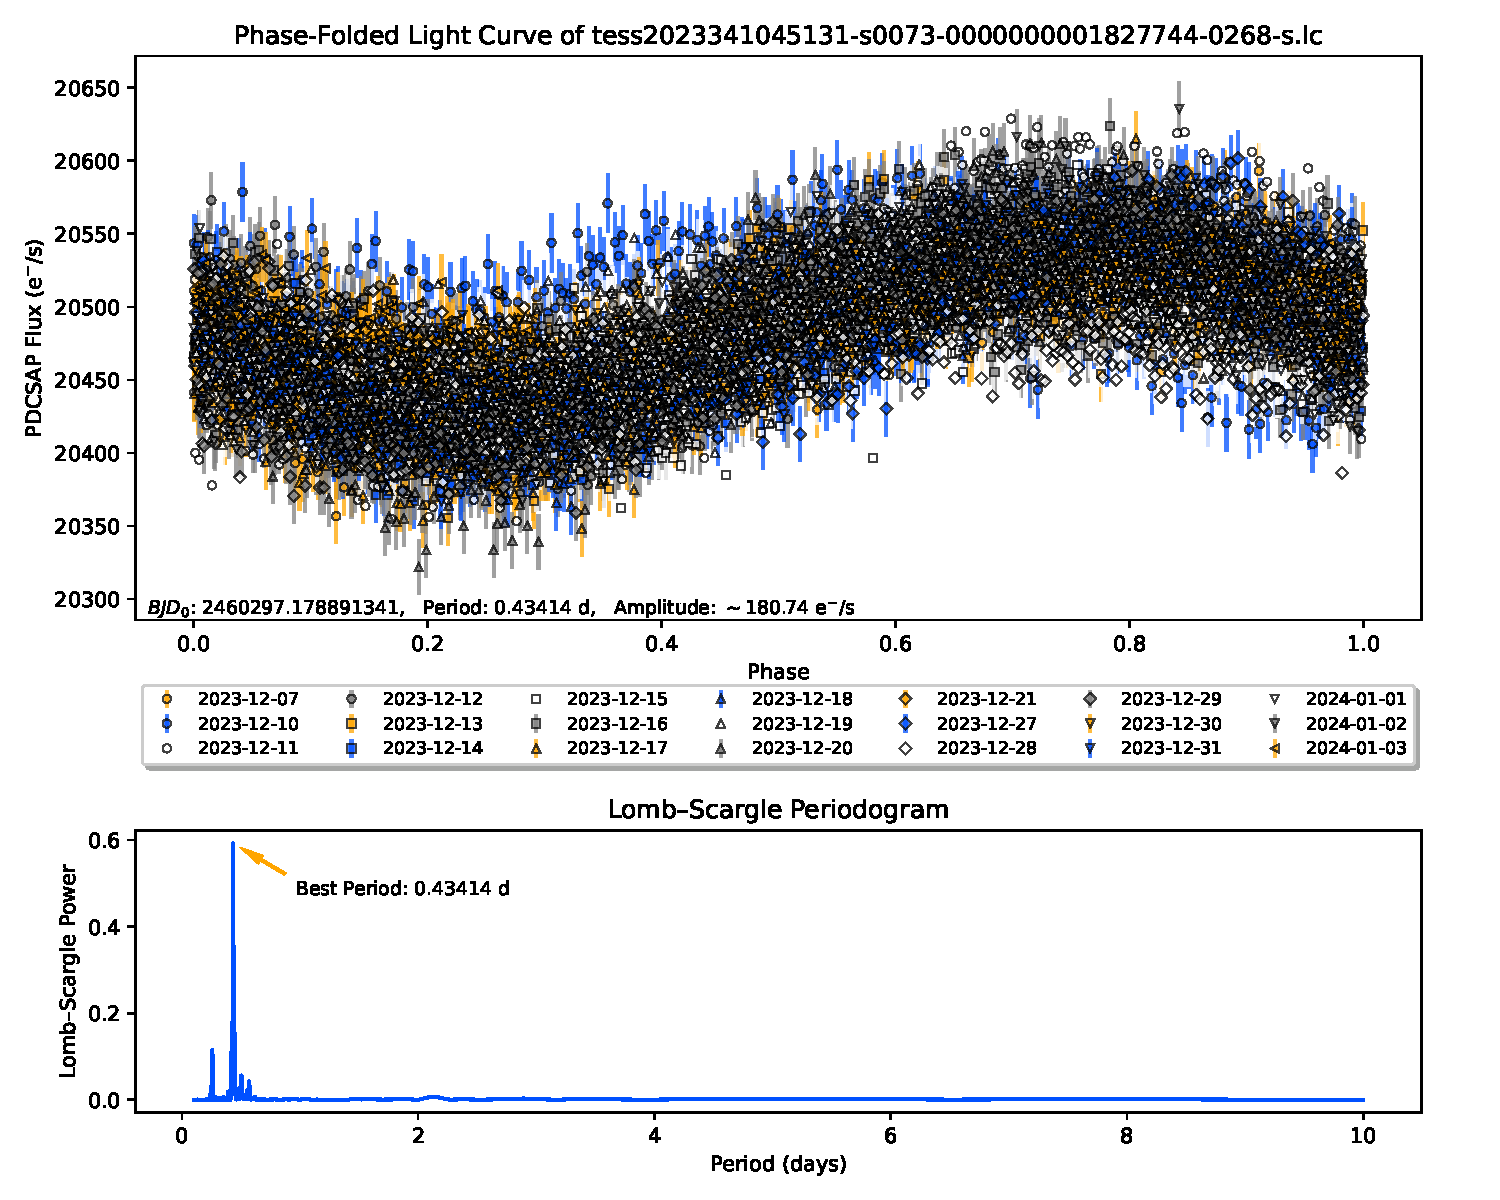
\includegraphics[width=\textheight]{figures/3-2.pdf}
  \end{frame}

  \section{Practice 4: Software Project Management \& Quality}
  \begin{frame}[t]{Software Project Management \& Quality}
    \textbf{Foundation:} Based on Lecture and Tutorial 8 \\\vspace{2.5mm}
    \textbf{Key Concepts Applied:} \\\vspace{2.5mm}
    \begin{itemize}
      \item \textbf{Version Control (Git \& GitHub)} \vspace{1mm}
      \begin{itemize}
        \item Creating and structuring GitHub repositories.
        \item Organizing project files (\rcode{/codes}, \rcode{/latex},
        \rcode{/csv}, etc.).
        \item Implied Git workflow (\rcode{git add}, \rcode{git commit},
        \rcode{git push}).
      \end{itemize} \vspace{1mm}
      \item \textbf{Documentation} \vspace{1mm}
      \begin{itemize}
        \item Importance of basic documentation for code and workflows.
        \item Role of \rcode{README.md} for project overview.
      \end{itemize} \vspace{1mm}
      \item \textbf{Software Testing} \vspace{1mm}
      \begin{itemize}
        \item Identifying test cases for functions (e.g., \rcode{get\_lc\_data},
        \rcode{fold\_lc}).
        \item Considering test scenarios (valid data, missing data, known
        periodicity, no periodicity).
      \end{itemize}
    \end{itemize}
  \end{frame}

  \begin{frame}[t]{Practice Showcase}
    \begin{itemize}
      \item \textbf{Practice 4:} Managing a project (GitHub repository set up)
    \end{itemize}
    \centering
    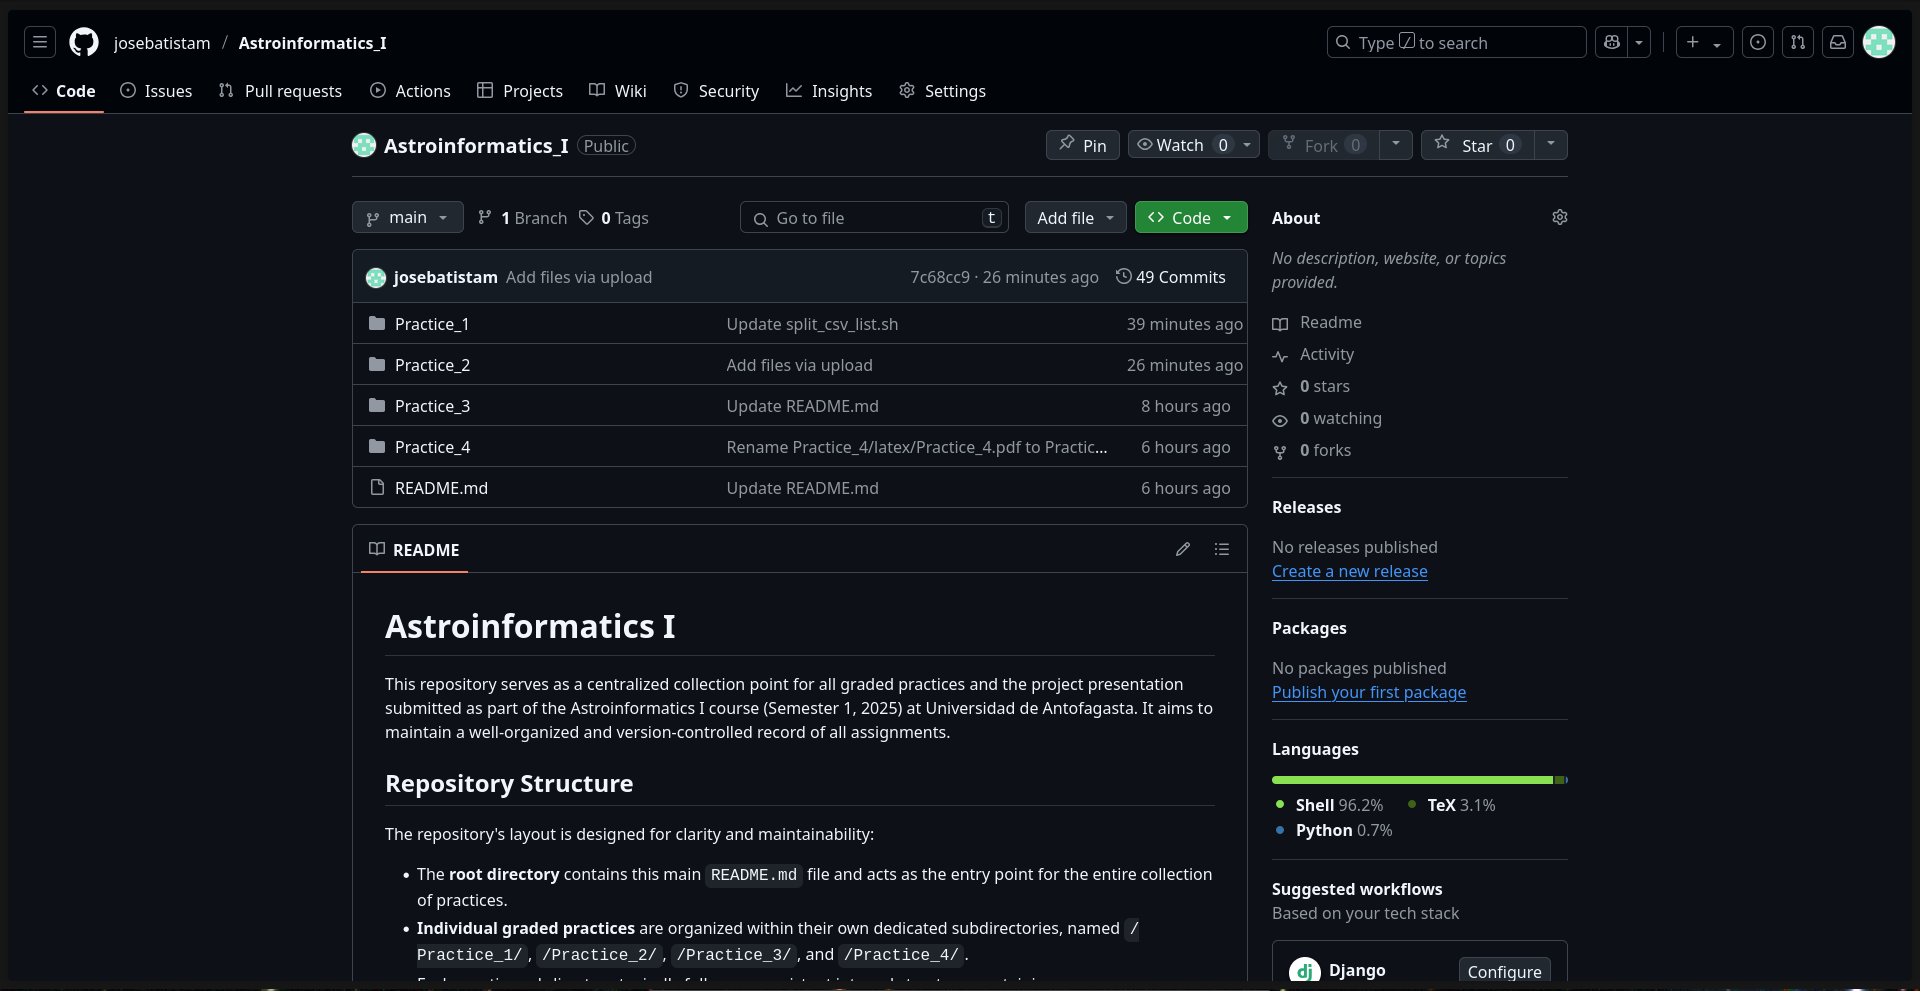
\includegraphics[width=1.5\textheight]{figures/4-1.png}
  \end{frame}

  \begin{frame}[t]{Practice Showcase (Cont.)}
    \begin{itemize}
      \item \textbf{Practice 4:} Managing a project (GitHub documentation creation)
    \end{itemize}
    \centering
    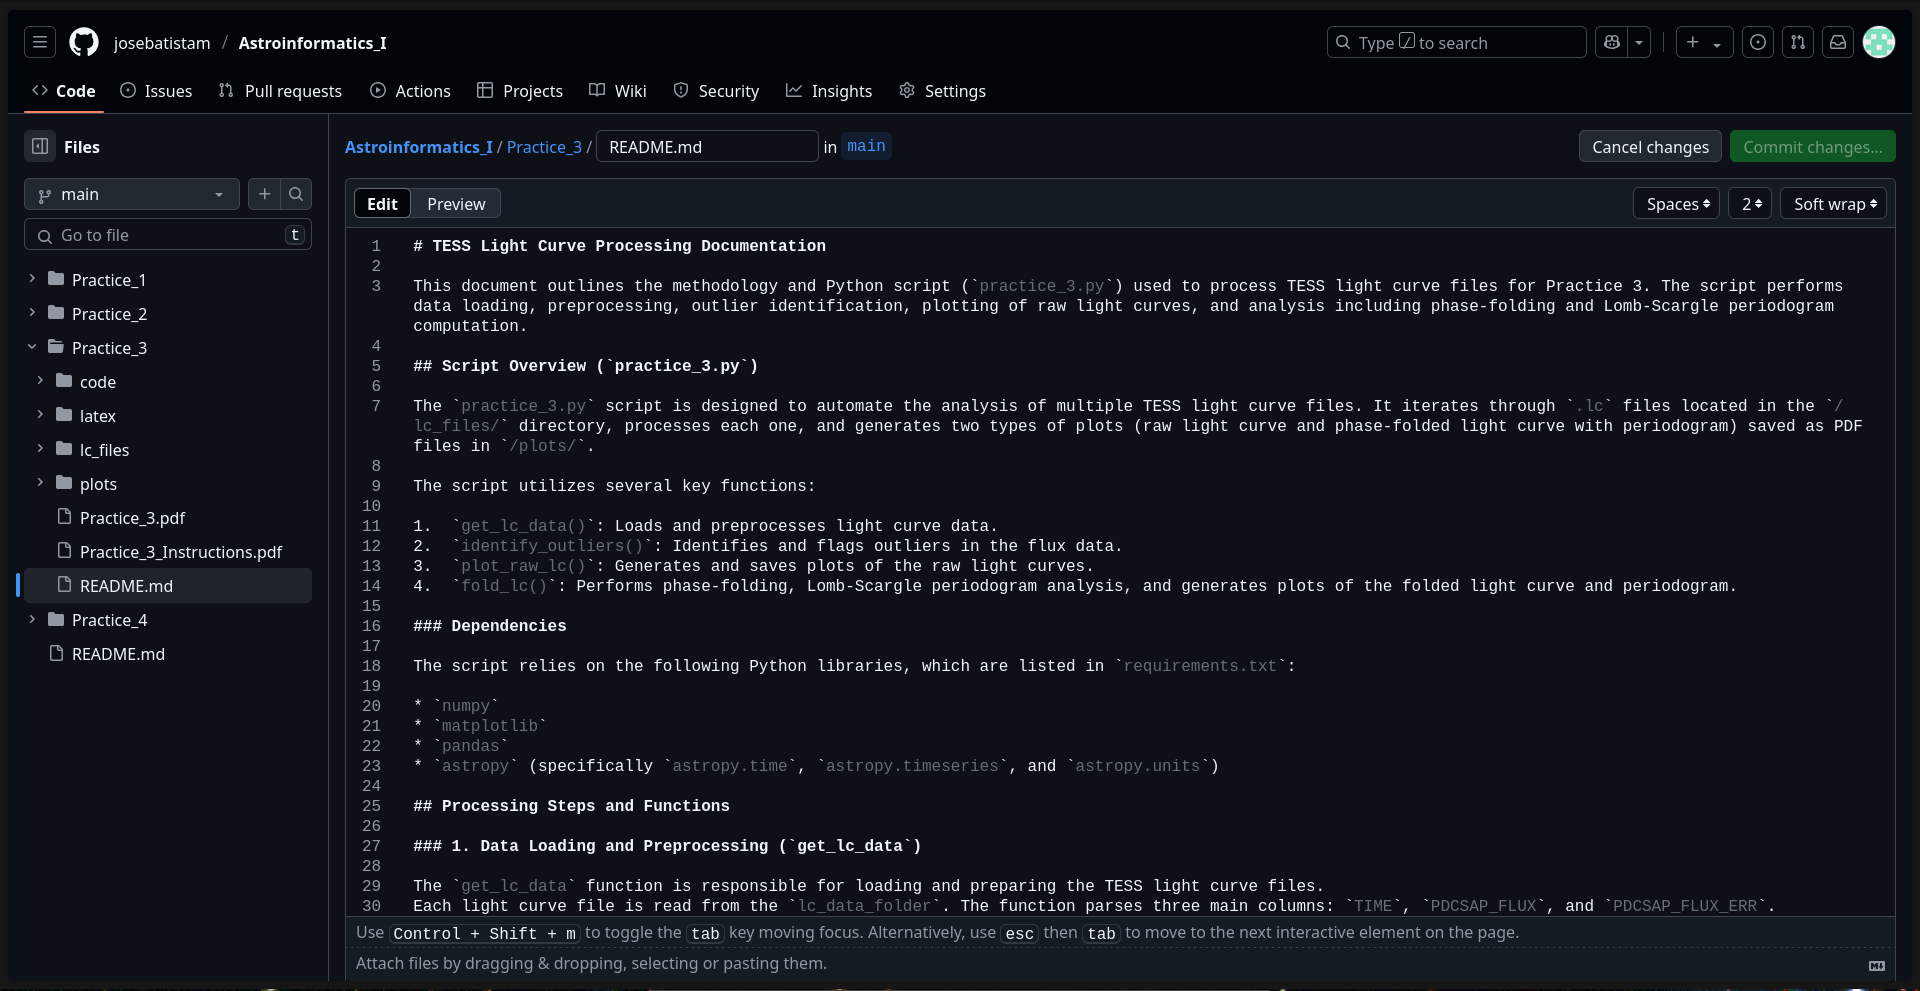
\includegraphics[width=1.5\textheight]{figures/4-2.png}
  \end{frame}

  \section{Conclusions}
  \begin{frame}[t]{Conclusions}
    \begin{itemize} \large
      \item The course succeeds in reinforcing the \textbf{interconnectedness} of seemingly disparate
      tools and principles. \vspace{2.5mm}
      \item Linux/Shell provides the essential command-line foundation
      for data wrangling, file management, and automating initial steps. It's
      the 'glue' that orchestrates tasks. \vspace{2.5mm}
      \item Python serves as the primary computational engine, allowing for
      sophisticated data analysis, algorithm implementation, and statistical
      modeling.
    \end{itemize}
  \end{frame}

  \begin{frame}[t]{Conclusions (Cont.)}
    \begin{itemize} \large
      \item Astronomical Libraries (Astropy, Lightkurve, etc.) bridge general-
      purpose Python with domain-specific astronomical knowledge, providing
      robust tools for units, time systems, and specialized analysis (e.g.,
      periodograms, phase-folding). \vspace{2.5mm}
      \item Software Engineering Principles (Version Control with Git/GitHub,
      Documentation, Testing) are paramount for ensuring that the code is
      \textbf{reproducible, maintainable, scalable, and collaborative}. They
      transform individual scripts into robust scientific tools. \vspace{2.5mm}
      \item Together, these elements form a powerful and synergistic toolkit,
      essential for navigating the complexities of modern astronomical data.
    \end{itemize} \vspace{2.5mm}
  \end{frame}

\end{document}